\section{Time Tracking Breakdown }\label{sec:time}

Below are summaries of the time we have spent on the project so far. A total for the team can be seen in \ref{fig:team}. The team has contributed over 309 hours so far to the project in eight weeks, if we keep that contribution up throughout the 12 week term we will have turned in around 425 hours which is quite a bit more than the minimum we planned for that period, which was 354 hours. 

\begin{figure}[H]
	\centering
	\graphicspath{ {./graphics/} }
    \centerline{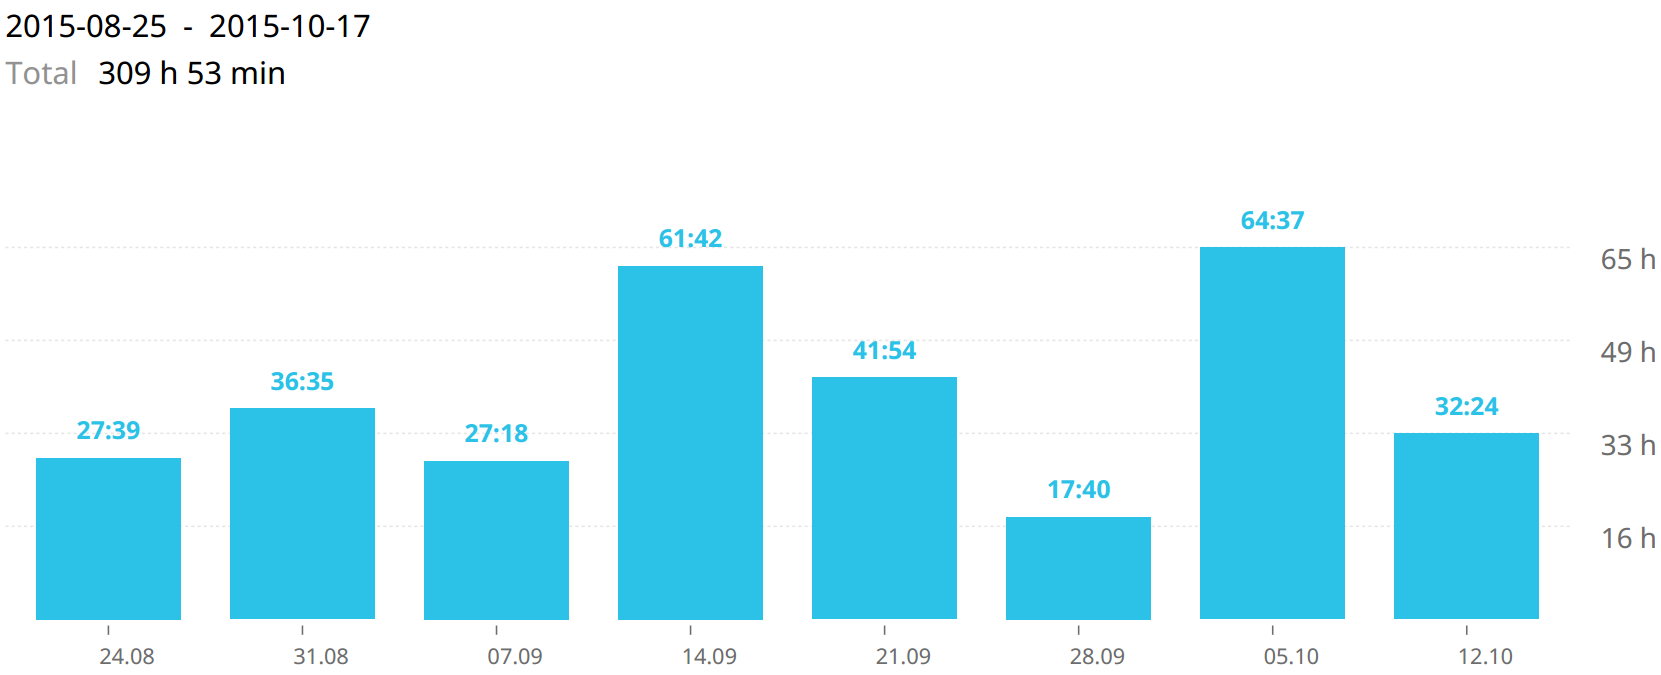
\includegraphics[scale=0.3]{teamtime.png}}
    \caption{\label{fig:team}Hours so far for the team}
\end{figure}

\begin{figure}[H]
	\centering
	\graphicspath{ {./graphics/} }
    \centerline{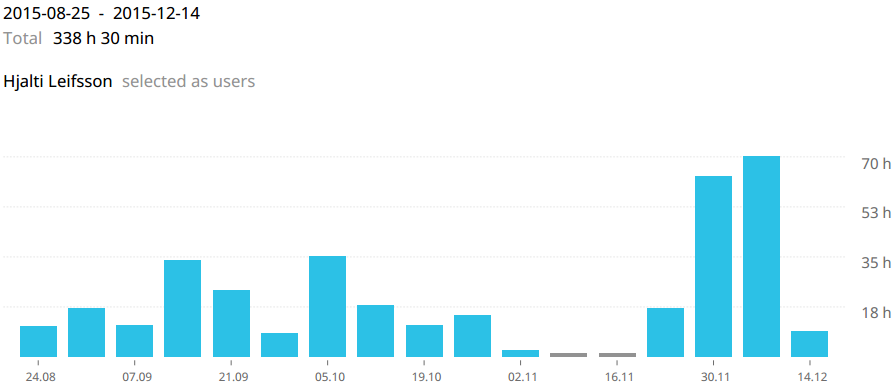
\includegraphics[scale=0.3]{hjaltitime.png}}
    \caption{\label{fig:hjalti}Hours so far for Hjalti}
\end{figure}

\begin{figure}[H]
	\centering
	\graphicspath{ {./graphics/} }
    \centerline{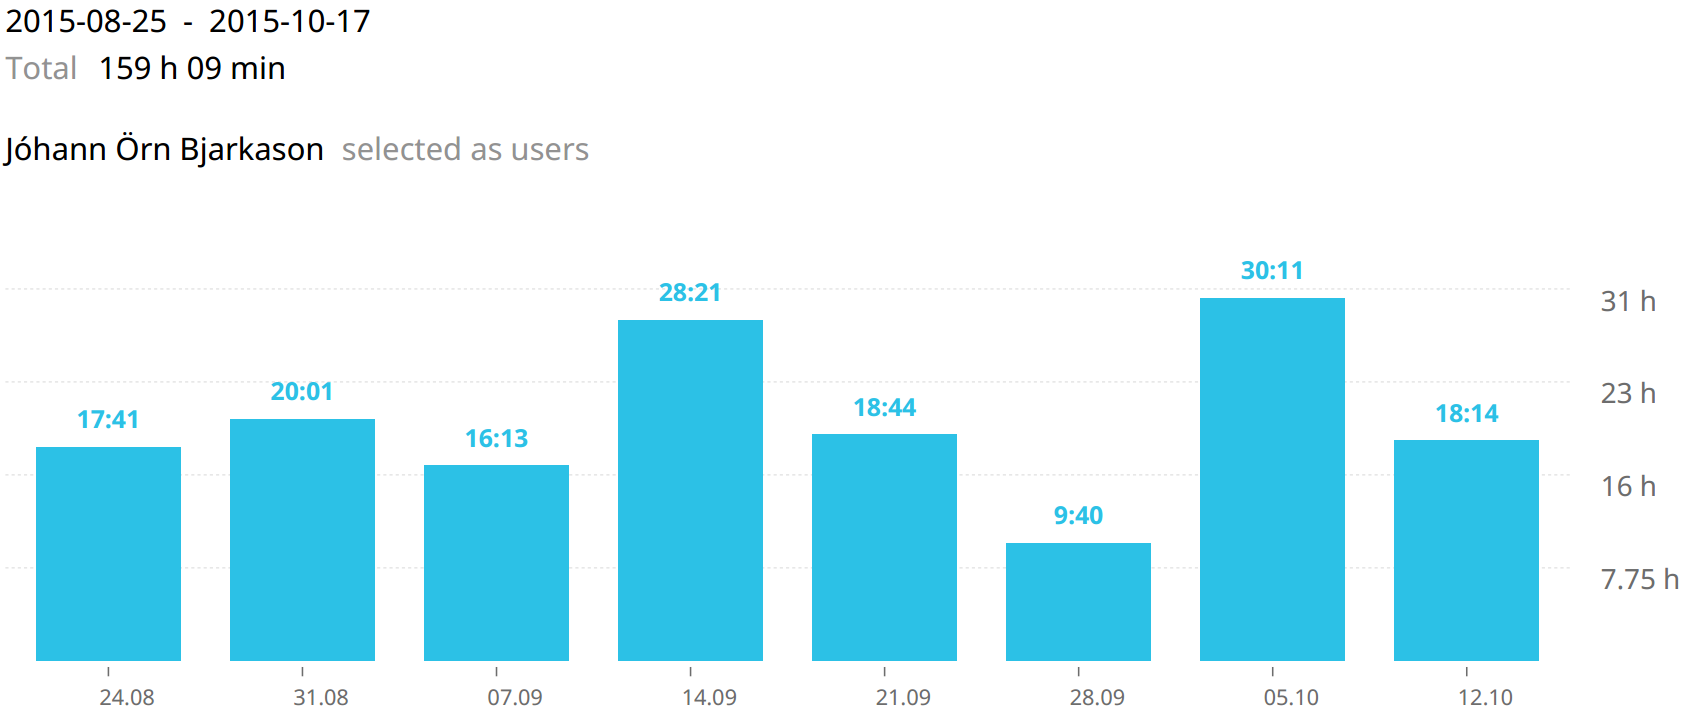
\includegraphics[scale=0.3]{johanntime.png}}
    \caption{\label{fig:johann}Hours so far for Jóhann}
\end{figure}

\begin{comment}
\noindent A breakdown of tasks can be seen in the following table:

\noindent
\addvbuffer[12pt 12pt]{\begin{tabular} {| l | c |}
	\rowcolor{LightSteelBlue}
	\hline Task description & Time spent \\
	\hline  Adding UI elements	&	25:09:05	\\
	\hline  Change Project Description report	&	1:32:14	\\
	\hline  Design review meeting	&	1:02:49	\\
	\hline  Design Review meeting	&	1:00:00	\\
	\hline  Figure out authentication errors	&	1:50:00	\\
	\hline  Fix delay in opening main UI	&	0:30:00	\\
	\hline  Fixing an error with the accuracy rating	&	0:38:35	\\
	\hline  Fixing bunch of little errors	&	5:38:53	\\
	\hline  Investigate delay in opening UI	&	0:30:00	\\
	\hline  Make a loading indicator for when the sample is loading	& 4:16:08	\\
	\hline  Making new API keys and error logging	&	1:00:00	\\
	\hline  Moving reports to the cloud	&	0:30:00	\\
	\hline  Organize sprint	&	1:20:00	\\
	\hline  Populating product backlog	&	5:38:00	\\
	\hline  Programming functionality	&	2:10:49	\\
	\hline  Risk analysis report	&	1:05:29	\\
	\hline  Scrum meetings	&	1:00:00	\\
	\hline  Showing the players accuracy rating on the header.	&	5:04:00 \\
	\hline  Sub-tasking stories for the sprint	&	1:00:00	\\
	\hline  Troubleshooting client problems	&	1:00:00	\\
	\hline  Troubleshoot Perforce	&	0:40:00	\\
	\hline  UI Design meeting	&	0:30:00	\\
	\hline  Updating and fixing the Product Backlog	&	2:00:00	\\
	\hline  Updating risk analysis and product backlog	&	0:36:00	\\
	\hline  Various meetings	&	5:35:02	\\
	\hline  Website meeting	&	0:30:00	\\
	\hline  Working on project Description report	&	1:00:00	\\
	\hline  Working on work schedule report	&	3:45:19	\\
	\hline  Work on product backlog	&	8:10:23	\\
	\hline  Writing progress report	&	2:15:00	\\
	\hline  Writing project description report	&	9:17:04	\\
	\hline  Writing Project Description report again.	&	8:34:46	\\
	\hline  Writing report on work schedule and procedure	&	7:48:34	\\
	\hline  Total & 112:38:10 \\

	\hline
\end{tabular}}
\clearpage
\end{comment}